\documentclass[sigconf]{acmart}

\usepackage{booktabs} % For formal tables
\usepackage{balance}
% Copyright
%\setcopyright{none}
%\setcopyright{acmcopyright}
%\setcopyright{acmlicensed}
%\setcopyright{rightsretained}
%\setcopyright{usgov}
%\setcopyright{usgovmixed}
%\setcopyright{cagov}
%\setcopyright{cagovmixed}

\usepackage{multirow}

% DOI
%\acmDOI{10.475/123_4}

% ISBN
%\acmISBN{123-4567-24-567/08/06}

%Conference
%\copyrightyear{2021} 
%\acmYear{2021} 
%\setcopyright{acmcopyright}
%\acmConference[SIGCSE '21]{Proceedings of the ACM Technical %Symposium on Computer Science Education}
%\acmBooktitle{Proceedings of the ACM Technical Symposium on Computer Science Education (SIGCSE '21)}
%\acmPrice{15.00}
%\acmDOI{10.1145/3287324.3287496}
%\acmISBN{978-1-4503-5890-3/19/02}


\newcommand{\gameNameNS}{``Game Name''}
\newcommand{\gameName}{\gameNameNS~}
\newcommand{\pwOne}{\gameName \emph{v.}1.0~}
\newcommand{\pwOneNS}{\gameName \emph{v.}1.0}
\newcommand{\pwTwo}{\gameName \emph{v.}2.0~}
\newcommand{\pwTwoNS}{\gameName \emph{v.}2.0}
\newcommand{\pwThree}{\gameName \emph{v.}3.0~}

\newcommand{\JA}[1]{\footnote{\textbf{JA: #1}}}

% Programming Cards
\newcommand{\I}{\texttt{Instruction~}}
\newcommand{\Ins}{\texttt{Instruction}}
\newcommand{\M}{\texttt{Method~}}
\newcommand{\Mns}{\texttt{Method}}
\newcommand{\Gr}{\texttt{Group~}}
\newcommand{\Grns}{\texttt{Group}}
\newcommand{\R}{\texttt{Repeat~}}
\newcommand{\Rns}{\texttt{Repeat}}
\newcommand{\Rx}{\texttt{Repeat-X~}}
\newcommand{\Rxns}{\texttt{Repeat-X}}
\newcommand{\V}{\texttt{Variable~}}
\newcommand{\Vns}{\texttt{Variable}}

\newcommand{\Ser}{\texttt{Search~}}
\newcommand{\Serns}{\texttt{Search}}
\newcommand{\Sort}{\texttt{Sort~}}
\newcommand{\Sortns}{\texttt{Sort}}

%Safety
\newcommand{\Anti}{\texttt{Antivirus~}}
\newcommand{\Antins}{\texttt{Antivirus}}
\newcommand{\Scan}{\texttt{Computer Scan~}}
\newcommand{\Scanns}{\texttt{Computer Scan}}
\newcommand{\Fire}{\texttt{Firewall~}}
\newcommand{\Firens}{\texttt{Firewall}}
\newcommand{\Over}{\texttt{Overclock~}}
\newcommand{\Overns}{\texttt{Overclock}}


% Malware
\newcommand{\Vi}{\texttt{Virus~}}
\newcommand{\Vins}{\texttt{Virus}}
\newcommand{\Ran}{\texttt{Ransomware~}}
\newcommand{\Ranns}{\texttt{Ransomware}}
\newcommand{\Spy}{\texttt{Spyware~}}
\newcommand{\Spyns}{\texttt{Spyware}}
\newcommand{\Trj}{\texttt{Trojan Horse~}}
\newcommand{\Trjns}{\texttt{Trojan Horse}}
\newcommand{\Mal}{\texttt{Malware~}}
\newcommand{\Malns}{\texttt{Malware~}}

% Hacking
\newcommand{\Hack}{\texttt{Hack~}}
\newcommand{\Hackns}{\texttt{Hack}}
\newcommand{\Buf}{\texttt{Buffer Overflow~}}
\newcommand{\Bufns}{\texttt{Buffer Overflow}}
\newcommand{\CSS}{\texttt{Cross-site Scripting~}}
\newcommand{\CSSns}{\texttt{Cross-site Scripting}}
\newcommand{\SQL}{\texttt{SQL Injection~}}
\newcommand{\SQLns}{\texttt{SQL Injection}}
\newcommand{\DoS}{\texttt{Denial of Service~}}
\newcommand{\DoSns}{\texttt{Denial of Service}}



% Areas
\newcommand{\MS}{\emph{Method Stack~}}
\newcommand{\MSns}{\emph{Method Stack}}
\newcommand{\Play}{\emph{Main~}}
\newcommand{\Playns}{\emph{Main}}
\newcommand{\Bns}{\emph{Bonus~}}
\newcommand{\Bnsns}{\emph{Bonus}}

\newcommand{\Hand}{\texttt{Player's Hand}}
\newcommand{\Prg}{\texttt{Program Editor}}
\newcommand{\Hist}{\texttt{Game History}}
\newcommand{\Goals}{\texttt{Gameplay Goals}}




% Modes
\newcommand{\B}{\emph{Beginner~}}
\newcommand{\BNS}{\emph{Beginner~}}
\newcommand{\Std}{\emph{Standard~}}
\newcommand{\StdNS}{\emph{Standard}}



\begin{document}

\settopmatter{printacmref=true}
\fancyhead{}

\title{\pwTwo}
%\titlenote{Produces the permission block, and
%  copyright information}
%\subtitle{A Card Game for Teaching Cybersecurity, Algorithms and Methods}
\subtitle{A Game-based Approach to Teaching Programming and Cybersecurity Concepts}
%\subtitle{Applying Game-based Learning for Teaching Programming and Cybersecurity Concepts}
%\subtitle{Learning Basic Programming and Cybersecurity Concepts through a Game-based Approach}



%\subtitlenote{The full version of the author's guide is available as
  %\texttt{acmart.pdf} document}

\author{Anonymized Author(s)}



%\author{John Anvik$^*$,\hspace{0.5em} Md. Hasan Tareque$^*$,\hspace{0.5em} Steven Deutokom$^*$ ,\hspace{0.5em} Maimoona Bashir$^*$ }
%\affiliation{%
% \vspace{0.5em}\institution{University of Lethbridge$^*$}
%}
%\affiliation{%
%  \institution{\{john.anvik,\hspace{0.2em}mdhasan.tareque,\hspace{0.2em}deutekom,\hspace{0.2em}maimoona.bashir\}@uleth.ca}
%}

% 
% % The default list of authors is too long for headers.
%\renewcommand{\shortauthors}{Anvik et al.}

\begin{abstract}
\gameName is a web-based card game designed to teach the fundamentals of computer programming and cybersecurity. Unlike previous games, \gameName provides an interactive program-language independent learning environment where the goal of the game is not to solve a maze. Based on informal comments and the results of a formal user study, a number of aspects of the game were revised. First, a number of cards were either removed or refined. Also, cards were added to introduce the programming concept of algorithms and the user interface was improved to provide more information about the players and the game state. Finally, two modes of play were introduced to provide players a learning path that allows for a more gradual introduction of programming language and cybersecurity concepts.  

\end{abstract}

%
% The code below should be generated by the tool at
% http://dl.acm.org/ccs.cfm
% Please copy and paste the code instead of the example below.
%
\begin{CCSXML}
	<ccs2012>
	<concept>
	<concept_id>10010405.10010489.10010491</concept_id>
	<concept_desc>Applied computing~Interactive learning environments</concept_desc>
	<concept_significance>500</concept_significance>
	</concept>
	<concept>
	<concept_id>10003456.10003457.10003527.10003528</concept_id>
	<concept_desc>Social and professional topics~Computational thinking</concept_desc>
	<concept_significance>300</concept_significance>
	</concept>
	<concept>
	<concept_id>10003456.10003457.10003527.10003531.10003533.10011595</concept_id>
	<concept_desc>Social and professional topics~CS1</concept_desc>
	<concept_significance>300</concept_significance>
	</concept>
	<concept>
	<concept_id>10003456.10003457.10003527.10003539</concept_id>
	<concept_desc>Social and professional topics~Computing literacy</concept_desc>
	<concept_significance>300</concept_significance>
	</concept>
	</ccs2012>
\end{CCSXML}

\ccsdesc[500]{Applied computing~Interactive learning environments}
\ccsdesc[300]{Social and professional topics~Computational thinking}
\ccsdesc[300]{Social and professional topics~CS1}
\ccsdesc[300]{Social and professional topics~Computing literacy}

\keywords{Programming language education; Cybersecurity education; Web application; Card game; Game-based Learning}

\maketitle
\section{Introduction}

Most games and environments developed with the intention of teaching computer programming concepts do so by requiring the student to either learn an existing programming language (e.g. Java \cite{Robocode}, Python \cite{CodeWars,CheckIO} or JavaScript \cite{CodeCombat,CheckIO,Codingame}) or a language specific to the learning environment (e.g. Scratch \cite{Scratch} or Alice \cite{Alice}). If the goal is to teach the fundamental concepts of computer programming, this requirement can result in a situation where the learner feels intimidated, confused or frustrated when their ``program'' does not work correctly. Also, as Bromwich et al. noted, many of these educational programming languages and environments are ``often ambitious in what they are trying to teach beginning programmers. They even go as far as to try teaching concurrency, something with which even advanced programmers often have difficulty.'' \cite{Bromwich2012}.

Also, such learning games and environments commonly use either a puzzle-solving premise, such as navigating a maze, or a sandbox paradigm, where a learner can utilize the language in an open-ended manner. As puzzle-solving activities tend to favour a specific demographic \cite{Phan2012}, and the sandbox paradigm requires oversight by an outside influence (i.e. an instructor) to ensure learning progression \cite{Bromwich2012}, both approaches have significant drawbacks.    

\gameNameNS
%\footnote{https://github.com/SibylLab/program-wars}
\footnote{Project repository URL removed for blind-review.} 
was created to address these concerns by providing a web-based card game that teaches or reinforces the fundamental concepts of programming and cybersecurity to those with limited or no programming or computer security experience \cite{anvikPW}. Players use various cards to create a program that executes a target number of instructions while launching cyberattacks against opponents and using representations of cybersecurity tools to defend themselves. Players are awarded additional points according to how they construct their program.

Several limitations and areas for improvement were identified for the initial version of \gameName following both formal \cite{anvikPW} and informal observations and discussions with players. The specific limitations identified included: confusion regarding the concept of method/function/procedure, the overgeneralization of cyberattacks, and frustration due to the randomness of the ``conditional statement" game mechanic.

This paper presents a redesign of \gameName which addresses these limitations, resulting in \pwTwoNS, a version which we believe better communicates the principles of functional decomposition, conditional statements, and real-world cybersecurity concepts. Also, \pwTwo introduces learners to two key classes of algorithms: searching and sorting.

The paper proceeds by presenting a survey of card or board games whose intent is similar to that of \gameName, followed by a description of the gameplay and cards found in \pwTwoNS.

\section[Related Work]{Related Work}
\label{sec:Related Work}

Several research works have been conducted regarding the use of games for teaching computer programming and software engineering.

The chapter illustrates the related research work as well as the related games that were developed for Game-Based Learning in SE.

\subsection{Game-Based Learning research in SE}
The following is an overview of the previous work regarding Game-Based Learning in the field of software engineering.

Tao et al. \cite{educational} emphasize learning software engineering through different gaming approaches. In their research, they found that gaming for software engineering education required a slightly different approach than the traditional Game-Based Learning methodologies. They created Pex4Fun to serve both the social aspects of Game-Based Learning and the presentation of software engineering content. The learning outcome from the research work is gaming and entertainment can be a source of education and that interactive learning has excellent value. Another discovery is that learning while playing can be effective in the industrial field.

Swapneel et al. \cite{halo} discussed how highly addictive socially optimized (HALO) provides concentration through an adaptive environment. The game environment is developed in such a way so that the player can enjoy the work in a gaming atmosphere. 
it for company uses. The initial stage is known as ‘Quest’, which is a preliminary introduction of the system. Here someone senior must work voluntarily or can be assigned. If the quest is harder for a single player, it could be done in a team, and then it is called a party. A simple quest can form a chain of quests, like use-cases or bug fixing. Another essential aspect is context switching. If an employer works on different modules then it will require more time, but HALO groups the same type of coding all together so that less context switching is required. In this process, a balanced environment has been created where players progress through multiple difficulties. The game is designed as a simple plugin to integrate with an IDE\footnote{Integrated Development Environment (IDE) is known as a software application that provides comprehensive facilities to computer programmers for software development.}, such as Eclipse or Microsoft Visual Studio. Making the user comfortable with the working environment is one of the significant contributions of HALO. A gamer is more comfortable in the gaming environment using this technique HALO adopted a context switching free environment. HALO is designed for the software industry, where the different projects have different requirements. Along with that is supports various social aspects like teamwork, project management.
Both the academic and industrial fields can be beneficial by adopting the game-based approach in software engineering.  Evaluation of the technique was not present, which is one of the drawbacks of this research.  

Miljanovic et al. \cite{robobug} discussed Robobug, a debugging technique through gaming in their research paper. Debugging is an essential tool in programming. Many good programmers struggle to find the bugs in a code segment. Debugging requires practice and patience; both might be difficult for a new programmer. Many computer science students struggle with debugging and feel left behind. Robobug presents different debugging techniques at different levels. It also has hints, which are very helpful for learning.

Szabo \cite{gamedev} proposed GameDevTycoon for teaching software engineering. Based on their work, there are thirteen different criteria for Game-Based Learning. GameDevTycoon covers most of the criteria. Gameplay analysis and software process models are simultaneously covered in the game. Three primary stages of software development are taught through the gameplay. The initial stage is known as the garage, the second stage is called team management, and the final stage is known as world domination. Each stage has separate responsibilities; for example, in the initial stage in software development, one should focus on the quality and latest research. As the project grows, team building is an additional responsibility that needs to be handled. When the project is in the saturation stage, new research works should be promoted so that the new technology can be cultivated. Again some small but significant issues regarding team bonding and employee workload also need to be adequately addressed in terms of good team bonding.

Pieper et al. \cite{SEMAT} presented a case study of the Software Engineering Method and Theory (SEMAT) to identify the educational outcomes in Digital Game-Based Learning. SEMAT is a part of the emerging OMG\footnote{The Object Management Group (OMG) is a computer industry standards consortium.} standard \cite{kernerl}. The case study shows that the evaluation of a developed integrated scenario can provide an in-depth analysis of the result. Nevertheless, the data was not sufficient to reach a conclusive decision regarding the pattern of learning. As a result, SEMAT was not referred to as a standard. The researchers state that if the study could be conducted in a broader spectrum (larger dataset), the result of the case study might be eligible for a conclusive outcome.

Mauricio et al. \cite{gamesforlearning} identified a different methodology that can be or is already applied in different interactive games for Software Engineering (SE) Game-Based Learning. Also, they explored different primary studies related to SE education, found the learning outcomes and mapped those outcomes to different SE project stages. 

Vladimir et al. \cite{gamification} discussed the different classifications of gameplay and their impact on several learning criteria. According to the researchers, gamification is a growing area in the business industry. The researchers emphasized the SWOT (Strengths, Weaknesses, Opportunities, Threats) framework \cite{swot} to find the learning criteria. However, they found that creating a software engineering Game-Based engine is a challenging task, one which programmers and industry should give a high priority. 

\subsection{Games for Learning Software Engineering}
Several games have been created for teaching the basics of programming. However, most of them are platform-oriented (i.e. only work on Windows) or target a specific programming language (e.g. C++ or Java). For learning the basics regarding computer programming, it is essential to understand the underlying logic and conceptual ideas. In this section, several types of games, especially board games, card games, desktop-based games and web-based games, are presented.

\subsubsection{Board Games}
Board games are a part of tabletop games where different components of the game can be moved on an adjacent surface or board according to some predefined rules \cite{boardgames}. The following are a couple of board games, which teach different aspects of computer programming.

Battle Bots v2 \cite{BattleBotsv2}  was inspired by the Robo Rally \cite{roborally} game. The required number of players for the game is between two and twenty. In the middle of the board, there is a repair center. Each player will start the game with twenty-two cards. Each move is divided into two groups: the programming round and the action round. In the programming round, players have to play the movement cards. In this stage, no action card can be played. In action round, there are five-phase where different action cards can be played along with movement cards. The player who survives the match wins the game. The main advantage of the game is that the players have to plan about the moves, which is an important programming concept, as in programming, it is essential to set the goal. A player can design his/her game plan depending on the other players’ moves or personal requirements. As a result, a fair amount of calculation is needed, which is very important in the logical aspect of computer programming. The game has no actual programming interface, which is one of the drawbacks of the game. 

Robot Turtles \cite{RobotTurtles} is a game to teach kids to code by using simple direction cards to move a specific coloured turtle. The main focus of the game is to get the coloured turtle to the same coloured jewel piece on the board. There are three instructions: forwards, rotate 90 degrees left and rotate 90 degrees right. There are also some obstacles where players might have to use different techniques to overcome the situation, and some unique cards are also introduced like fire cards for shooting. The higher the level, the more complex cards need to be used.
Regarding programming, the jump card is the most crucial one. The idea of jump cards is that they can be replaced with a set of instruction cards that can be used repeatedly. There is also a bug card that can undo the immediate move the player has made. Robot Turtles is designed for kids’ initial steps in programming, like single statement compilation, which is well executed through a single card movement. The introduction of a jump card is an excellent initial concept of function calls. Bug cards introduce the idea of mistakes in programs.

Code Master \cite{CodeMaster} is a single person puzzle game that teaches logical problem-solving. There are sixty levels in the game with several challenging levels. The game consists of a map that has six different levels ranging from easy (green) to expert (red). There is also a guide scroll that indicates the order in which the program statements should run. Also, the guide has places for conditional tokens. There are three colours: green, blue and red. For each path, there is a specific token related to the colours. Numerical numbers are represented in the map nodes. The goal is to get to a portal and collect crystals using a limited path and moves. The game focuses on the programming construct of conditional statements (i.e. if-else). Some nodes have a self-loop, which illustrates the concept of a repeat statement. Finally, the shortest path selection is also a focus point. The game requires essential thinking before each move, which is vital for developing logical thinking. Unidirectional and bi-directional edges in a graph can be learned by playing the game. 

\subsubsection{Card Games}

A card game can be defined as a game that involves different playing cards as the main components with which the game can be played \cite{cardgames}.

Potato Pirates \cite{PotatoPirates} was the only physical card game found that intends to teach programming concepts. The main objective of the game is to make the user familiar with different programming concepts through social interactions. The final goal of the game is to achieve seven specific cards, named Potato King, through different logical actions performed through different cards. To win the game, a player needs to eliminate all the other ships in possession of the other players or acquire all seven Potato Kings by drawing them from the deck or by eliminating other players’ ships and seizing their cards. Players can power up their attacks with programming concepts cards such as loops and conditionals. The game covers the concepts of programmings such as variables, functions, while-loops, if-else conditionals and nested-loops. Some surprise cards serve the purpose of interrupts and control flow. The game illustrates the branching condition very nicely, which is equivalent to the if-else statement. The use of variables is well defined. Different repeat structures are also presented in a reasonable manner such that the game covers the loop structure of programming languages. There is also an option for creating a loop inside a loop, which is known as a nested loop. The game also covers the case structure (switch case or nested if-else).

\subsubsection{Web-based Games}

Games that can be played on the World Wide Web are known as web-based games. These games use standard web technologies or browser plugins \cite{webbasedgames}.

CodeCombat \cite{CodeCombat} is a web-based game focusing on learning JavaScript, Python, and other programming languages. The game is built upon concepts of swords-and-sorcery where the player has to role-play as a warrior. The main objective of the game is to learn necessary programming skills by overcoming different challenges like clearing the maze, picking up gems and avoiding any spikes or attacking ogres. The gameplay is split between a code editor on the right and a simulation effect on the left. Figure \ref{fig:CodeCombat} shows the interface of the game. The avatar is controlled by using a set of commands.  In each level, the player has to accomplish a set of tasks. As the game progresses, the player is gradually introduced to new concepts like loops, conditionals, and variables. If a person does not have programming experience, CodeCombat is very suitable. As the game progresses, the tasks involve more complex programming concepts. Most importantly, the levels themselves become more complicated due to possible interactions with the objects in the game world.\\

\begin{figure}[ht!]
	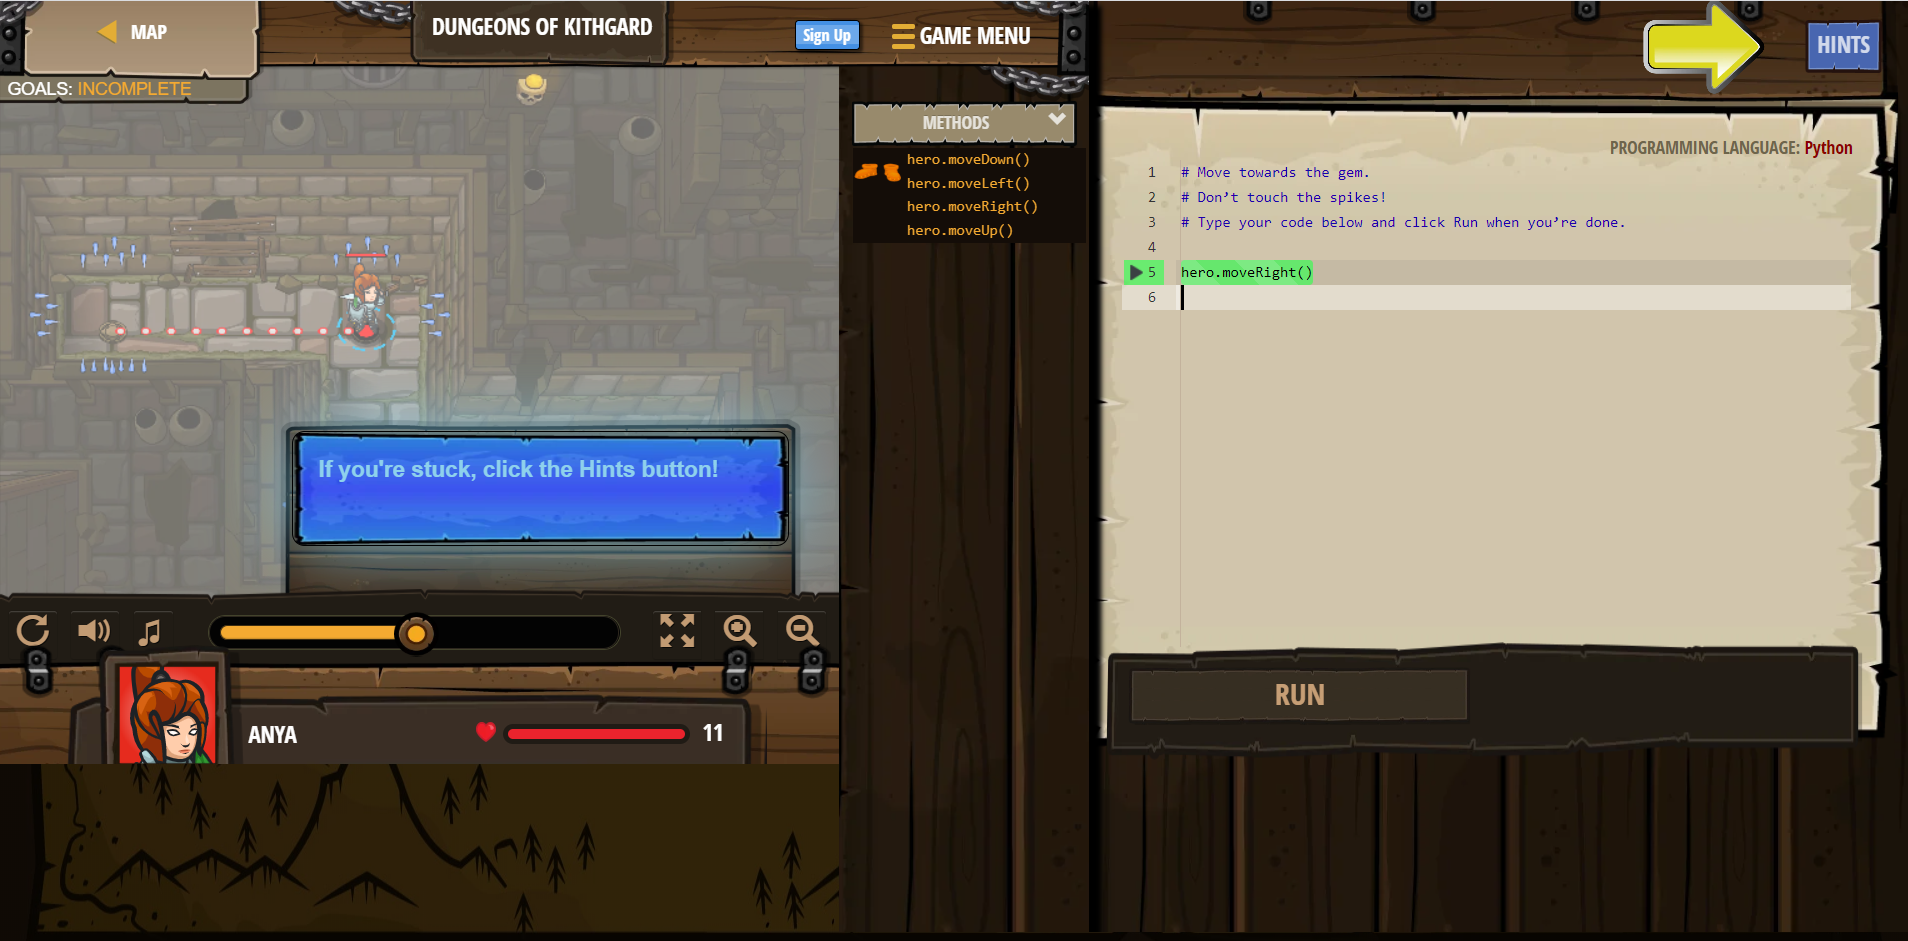
\includegraphics[width=\columnwidth]{images/CodeCombat.PNG}
    \caption{CodeCombat gameplay}
    \label{fig:CodeCombat}
\end{figure}

Blocky maze \cite{Blocklymaze} is a game that introduces the concept of programming loops and conditions in Javascript without writing any Javascript code. The game is a combination of levels that teach programming. It is designed for children who have not had prior experience with computer programming. The game uses a graphical programming language implemented in JavaScript, which can compile to JavaScript, Dart or Python. In the game, programming is done by dragging and dropping code blocks onto a design surface. Figure \ref{fig:BlocklyMaze} shows the interface of the game. The main objective of the game is to take the avatar from a starting point to the endpoint. There are a total of ten levels, and the complexity increases as the game progress. Some goals are set to solve the maze in a particular number of steps, which is also challenging. The game interface is similar to a Google Map, which might help the user to adopt the game. 

\begin{figure}[ht!]
	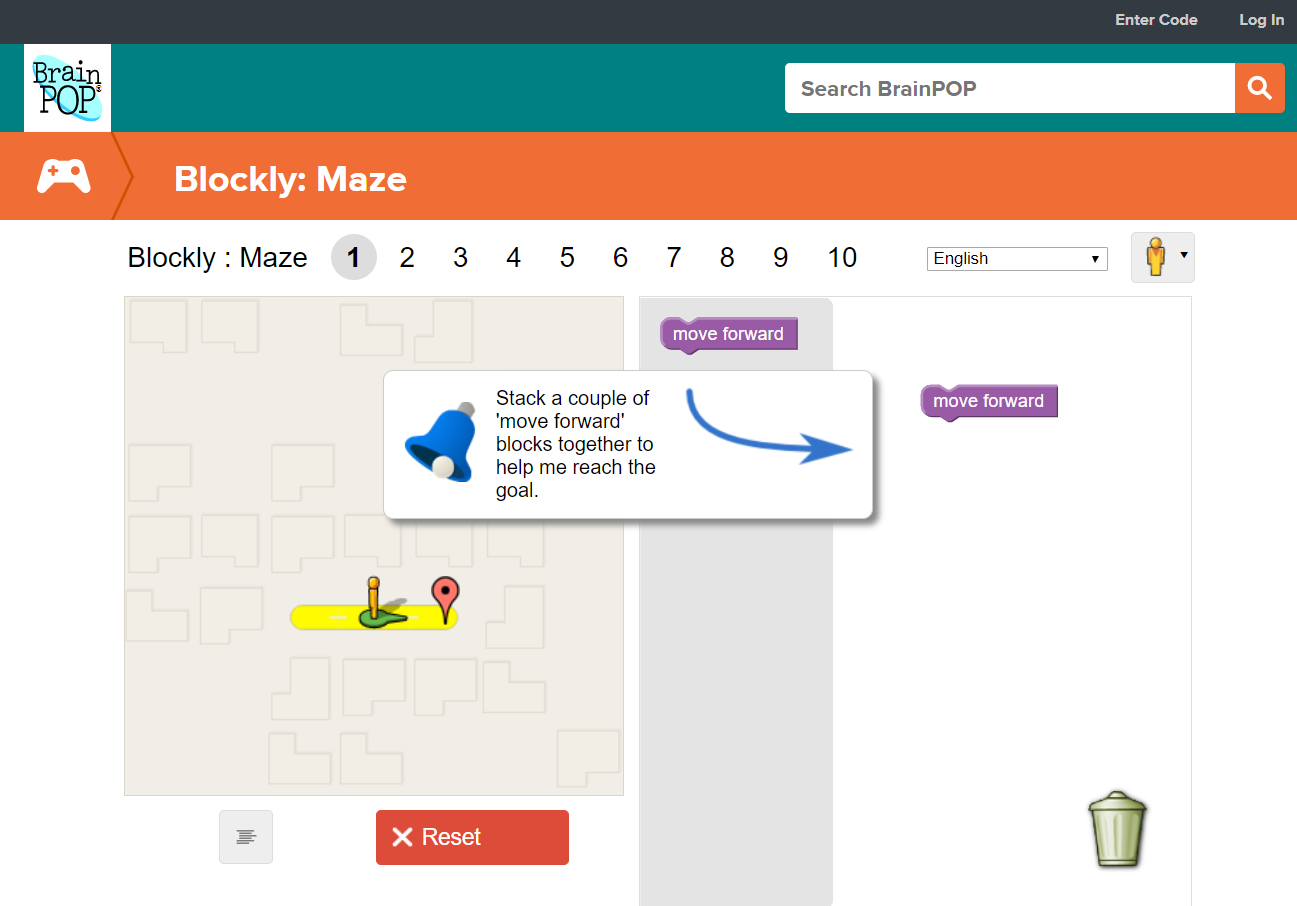
\includegraphics[width=\columnwidth]{images/BlocklyMaze.PNG}
    \caption{Blockly Maze gameplay}
    \label{fig:BlocklyMaze}
\end{figure}

CodinGame \cite{Codingame} supports many programming languages. The main objective of the game is to improve players’ coding skills by solving different problems, applying new strategies and getting inspired by other strong opponents. The game can be played in single and multiplayer mode, which gives it the feeling of fun rather than learning. A player can choose any programming language among more than twenty, such as Python, Ruby, Java, and Scala. The targeted group for the game is the people who have basic programming knowledge as well as expert developers. In the game, users create a profile, which is used for challenges and contests. There are opportunities for players to make their profile public so that employers can find them to offer them a job. Also, the game has a forum for members to chat about languages, questions, and share information. The game is not for beginners because it requires some basic knowledge of programming. Figure \ref{fig:CodinGame} shows the interface of the game.

\begin{figure}[ht!]
	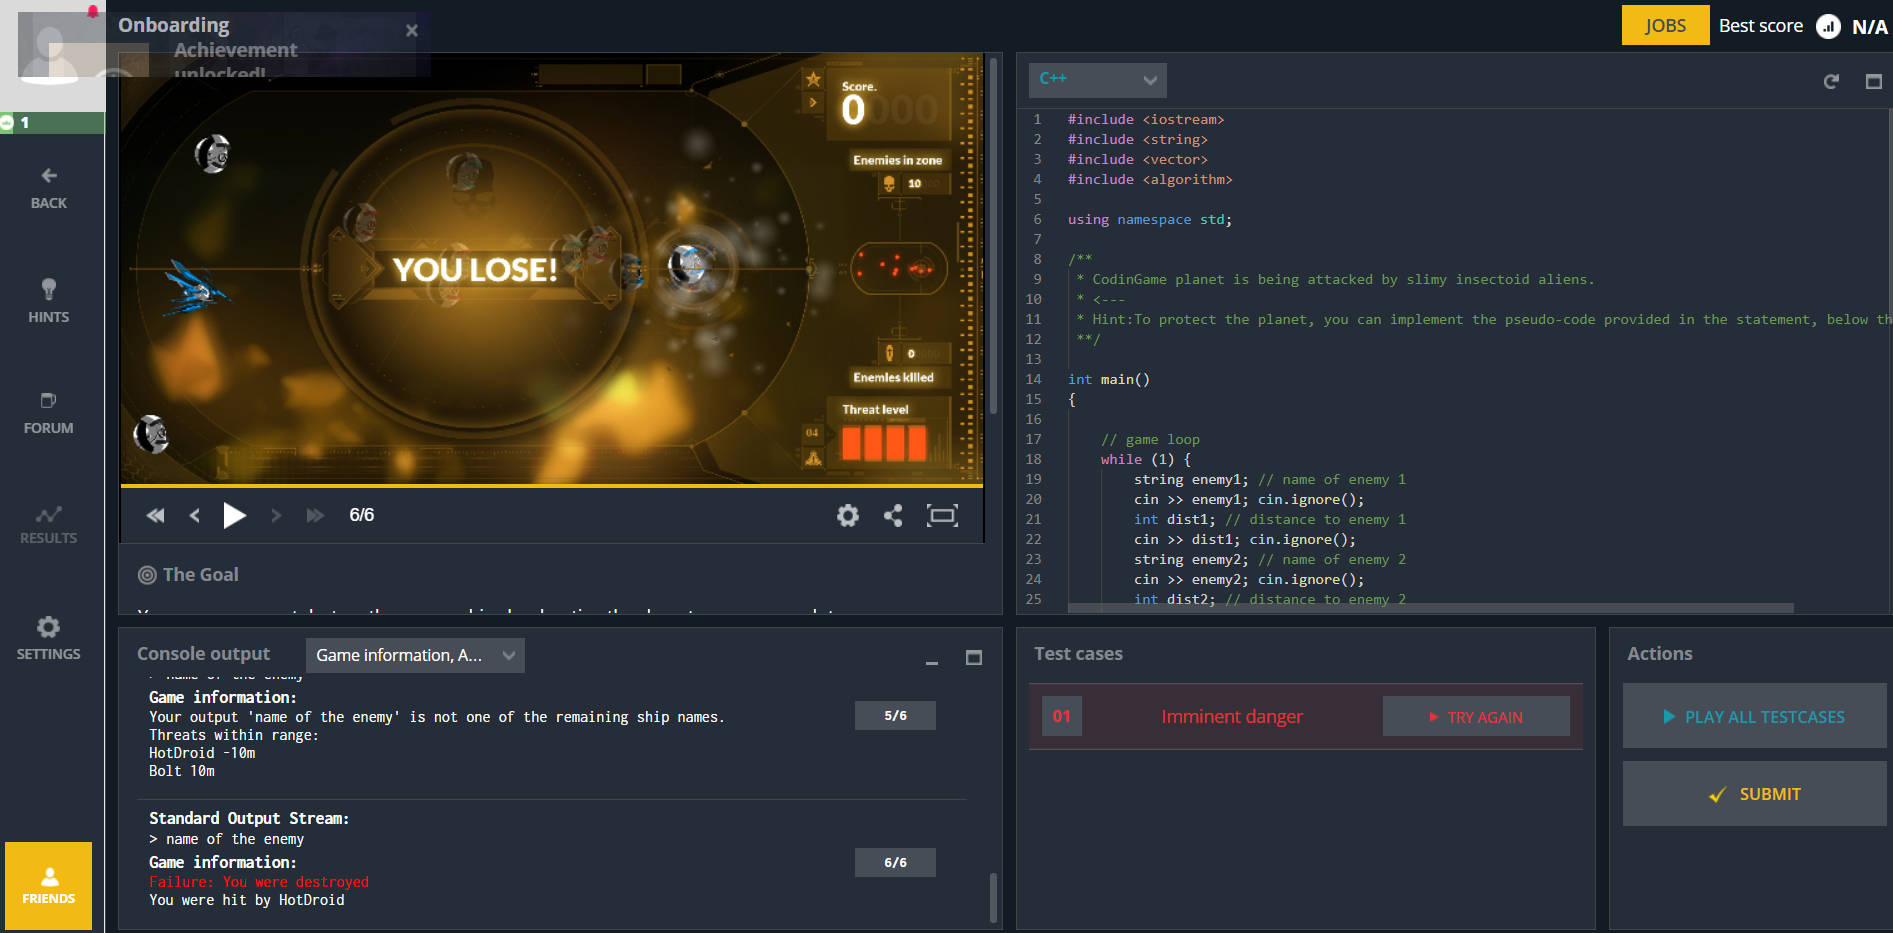
\includegraphics[width=\columnwidth]{images/CodinGame.PNG}
    \caption{CodinGame gameplay}
    \label{fig:CodinGame}
\end{figure}

\begin{figure}[hbt!]
  	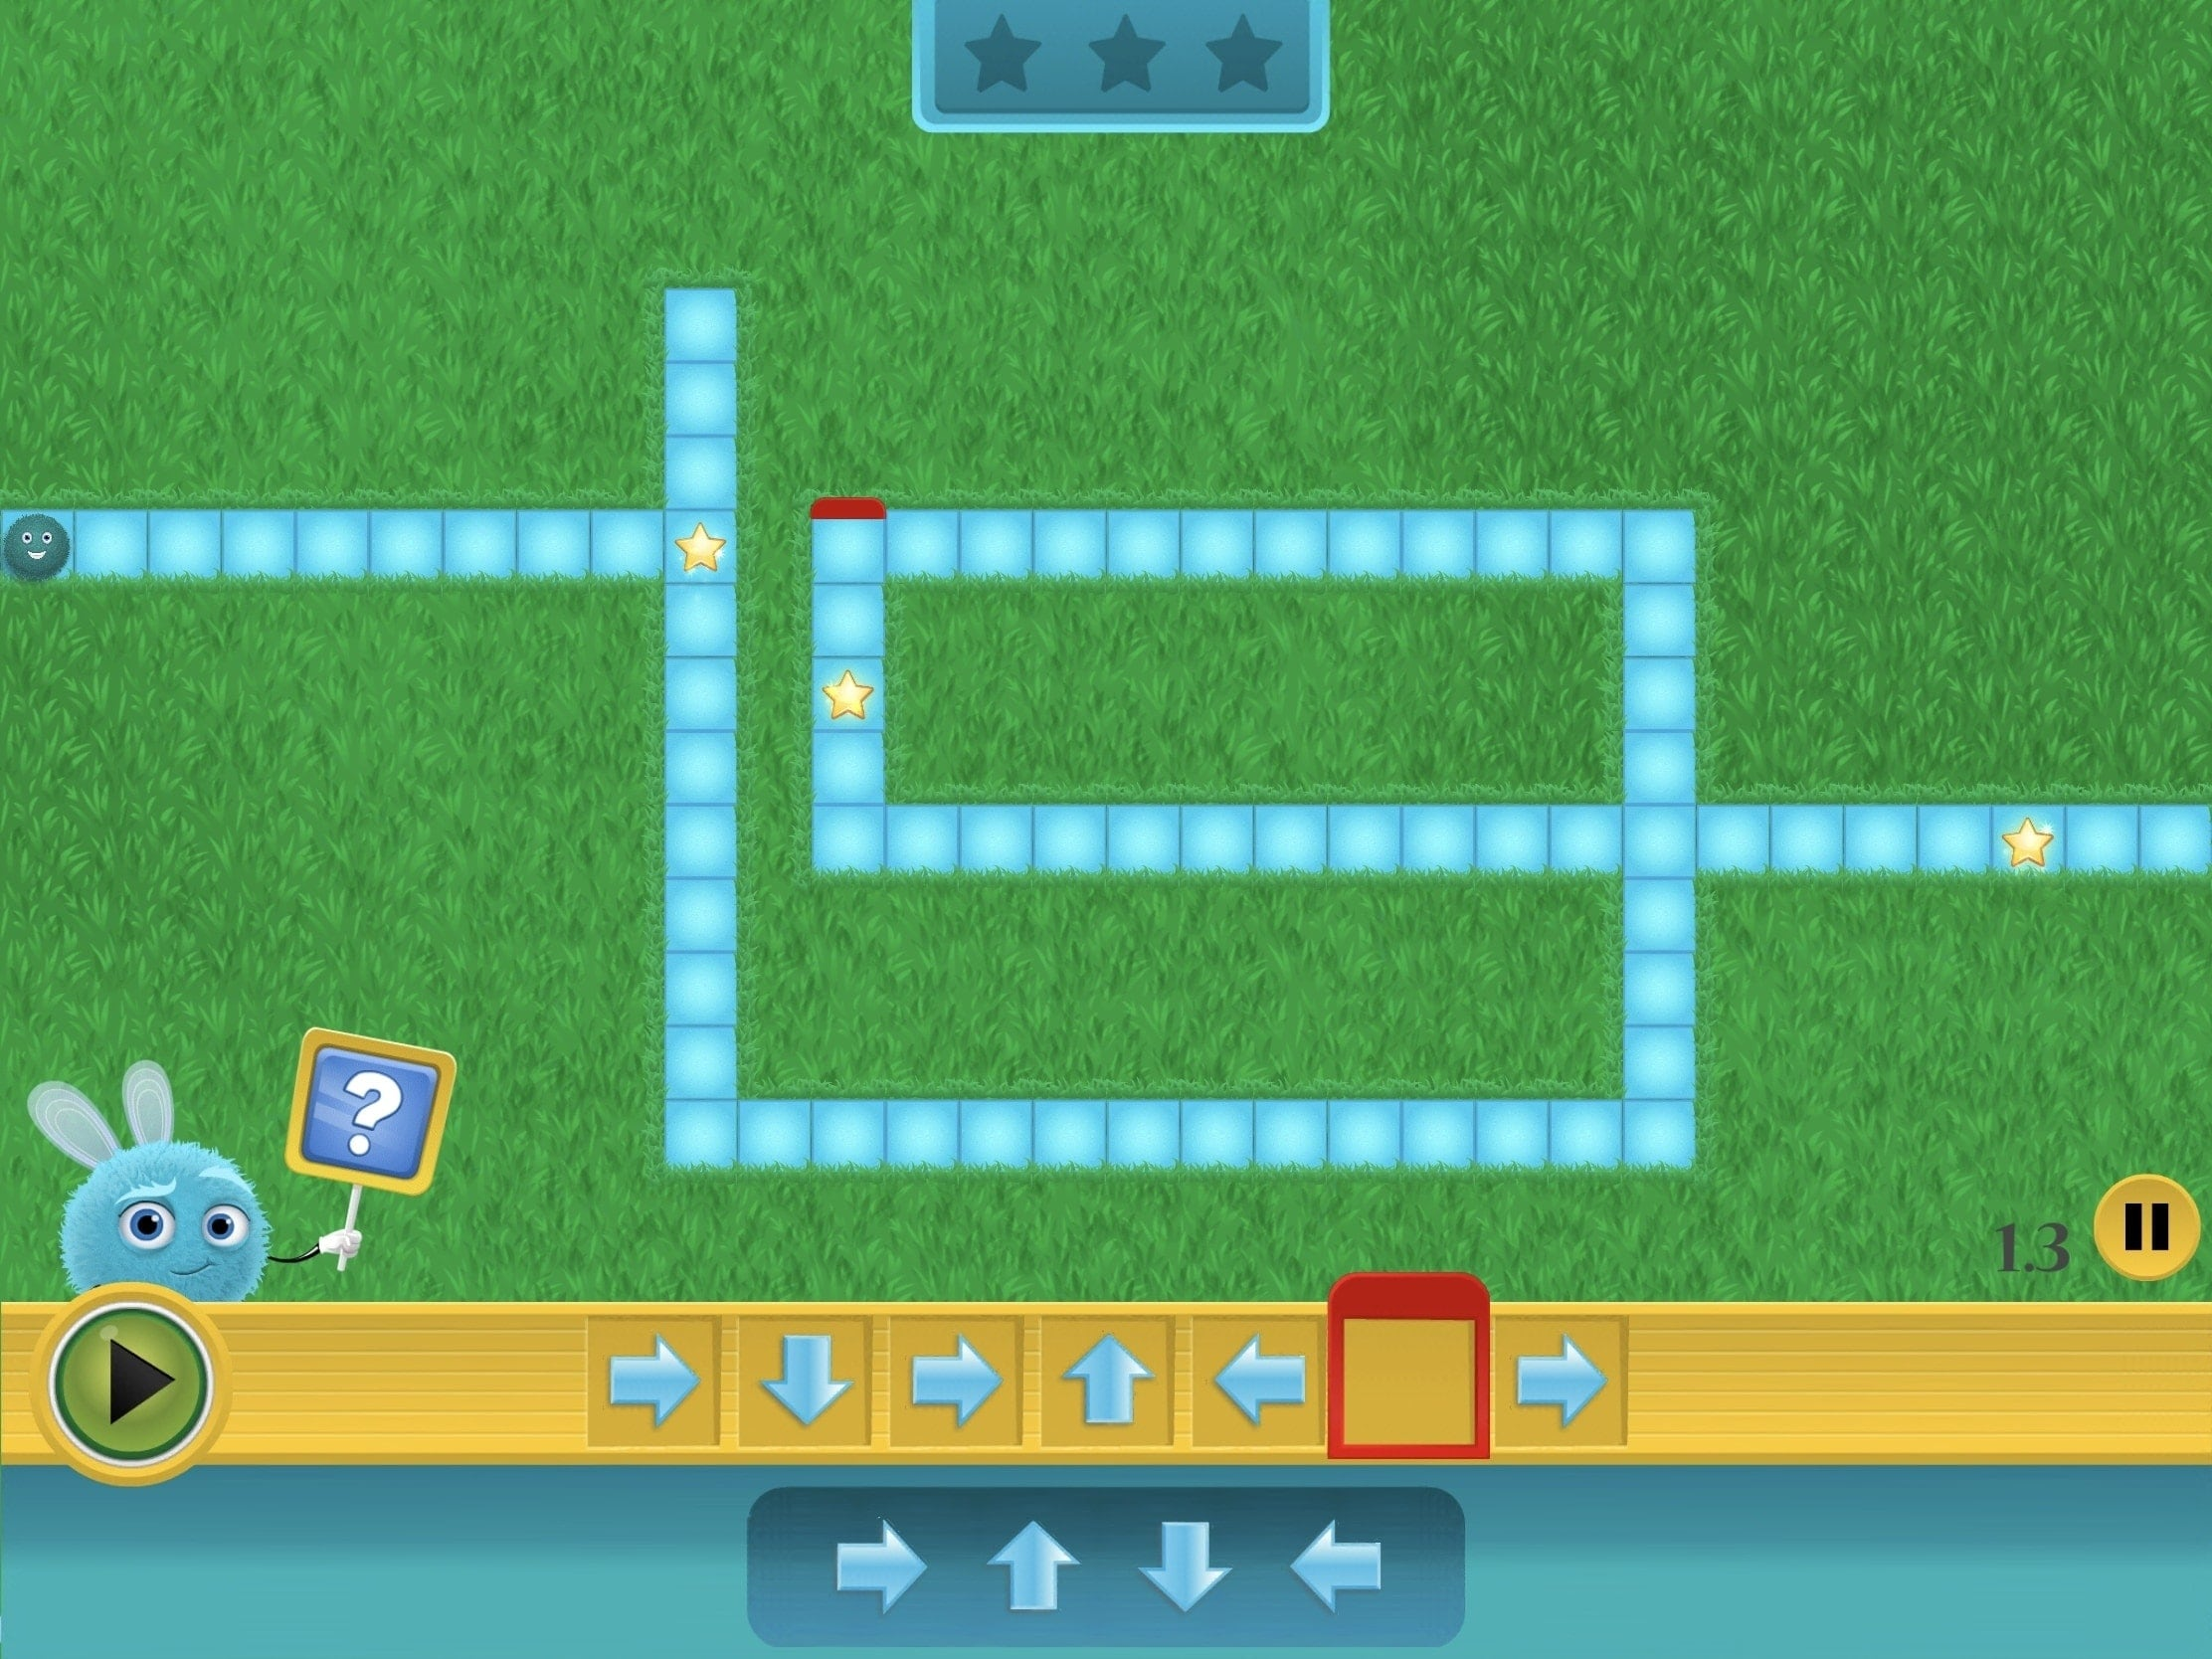
\includegraphics[width=\columnwidth]{images/Kodable.PNG}
    \caption{Kodable gameplay}
    \label{fig:Kodable}
\end{figure}

Kodable \cite{Kodable} is a game developed for kids that focuses on introducing logic and the decisions (i.e. if-then-else) in computer programming. Kodable’s programming language introduces players to step-by-step statements with different instructions using in the programming language. The primary programming concepts of conditional statements and loop structure, is well defined in the game. The social aspect of the game is presented into a parents section with written teaching instructions that assist the parent to unlock different levels for kids and extend logic skills into real life. The game is comprised of many features that are appropriate for children. The activities in the game help the player to think like a programmer, solve different problems and eventually to writing real code using the game’s custom coding interface. Figure \ref{fig:Kodable} shows the interface of the game. For logic development, the game focus on learning the importance of statement sequence. The game introduces kids to different types of data, such as integers and strings, and data structures, such as arrays. Finally, object-oriented programming concepts are also introduced by the game. 


Program Wars \cite{ProgramWars} is a web-based card game. The game focuses on learning programming and cybersecurity concepts. The player’s objective is to achieve a specific number of points through different cards. The game is platform-independent, which means that it is not focused on any single programming language. Instead, the game helps to develop an understanding of the underlying logic of programming. Here the players do not have to be concerned about syntax errors, and programming terms are being described using an elementary vocabulary. In Chapter \ref{ch:Overview of Program Wars}, a more detailed analysis regarding Program Wars is presented.   

%\section{Summary}
%Based on the related research works examined, practical implementation (i.e. learning a real programming language) and visualization of program results are essential in software engineering education. Also, learning through gameplay has more sustainable effects\cite{effectivenessofgames}. The main challenge of Game-Based Learning for software engineering is to maintain a balance between learning and engagement \cite{educationalgamedesign}. The gameplay should be presented in a structured way such that the user can relate the outcome to real-world programming. Most of the research deals with a specific part of a software engineering like debugging, the user interface, and project management.
%\section{Board and Card Games That Teach Programming}

This section provides a survey of other efforts for teaching computer programming where the medium used is a card game or a board game. 
Based on these works, we found that practical implementation (i.e. learning a real programming language concept) and visualization of a program's results are essential elements in learning computer programming. Also, we found that although learning through gameplay may have more sustainable effects \cite{effectivenessofgames}, the main challenge is that of maintaining a balance between learning and engagement \cite{educationalgamedesign}. Finally, the gameplay needs to be presented in a structured way such that the user can relate the outcome to real-world programming.

\paragraph{Potato Pirates:}
Potato Pirates \cite{PotatoPirates} is perhaps the most similar game to \gameName in intention and execution. It is a physical card game that intends to teach all the essential programming concepts. The premise of the game is that the player is a potato who captains a pirate ship, and the player conducts naval battles to sink the other player's ships and assimilate their crew. The goal of the game is to acquire seven ``Potato King" cards by performing different actions with playable cards. By playing the game, the user becomes familiar with different programming concepts. Players can power up their attacks with cards that represent loops and conditionals. This includes cards to represent different structures such as for-loops and while-loops, as well as an option to create nested-loops. Some cards introduce the concepts of interrupts and control flow. Finally, the game covers the concepts of variables, functions, if-else conditionals, and the switch-case construct.

\paragraph{Battle Bots v2:}
Battle Bots v2 \cite{BattleBotsv2}  was inspired by Robo Rally \cite{roborally}. In the game, each move is divided into two groups: the programming round and the action round. In the programming round, players play movement cards to move their ``bot" around the board. In the action round, there are five phases where different action and movement cards can be played. A player who survives the attacks from their opponents wins the game. Players need to design their gameplay according to the other players’ moves or personal requirements. The game teaches the logical aspects of computer programming through the players need to plan their moves. One of the game's drawbacks is that it has no actual programming interface. Also, it can be hard to understand how the game is to be played as we found that the description of the rules is not very clear.


\paragraph{Robot Turtles:}
Robot Turtles \cite{RobotTurtles} is a game that teaches computer programming by using simple direction cards to move a coloured turtle and is intended for pre-school age children. The game's objective is to move a coloured turtle from a square on the edge of the board to a square with a jewel matching the turtle's colour. The game's use of a single card for either directional or rotational movement of the turtle works well to simulate single statement programming instructions. This is effective at providing children with their first look at programming. Additionally, Robot Turtles introduces the concept of function calls with the \texttt{Jump} card which can be used to replace a set of instruction cards. These replaced cards can then be used repeatedly. Finally, the game introduces players to debugging through a \texttt{Bug} card that can be added to a player's program to indicate that it has a problem.

\paragraph{Code Master:}
Code Master \cite{CodeMaster} is a single-player puzzle game that teaches logical problem-solving. The goal of the game is to traverse a graph from a starting node to a destination node while using different moves to collect crystals along the way. The game introduces a player to the programming constructs of conditional statements (i.e. if-else), repetition (some nodes have a loop) and finding the shortest path. One of the game's primary focuses is critical thinking, which is a necessary skill for computer programming.

\paragraph{Blocky Maze:}
Blocky Maze \cite{Blocklymaze} is designed to teach the concepts of loops and conditions to players with no prior computer programming experience. The game uses a visual programming language that can be compiled into either JavaScript, Dart or Python to execute the program. In the game, programming is done by dragging and dropping code blocks onto a design surface. The main objective of the game is to take the player's avatar from a start point to an endpoint. The game is made up of a total of ten levels which increase in complexity as the player progresses.


\section{\pwTwo}

\begin{figure*}[ht]
	\centering
	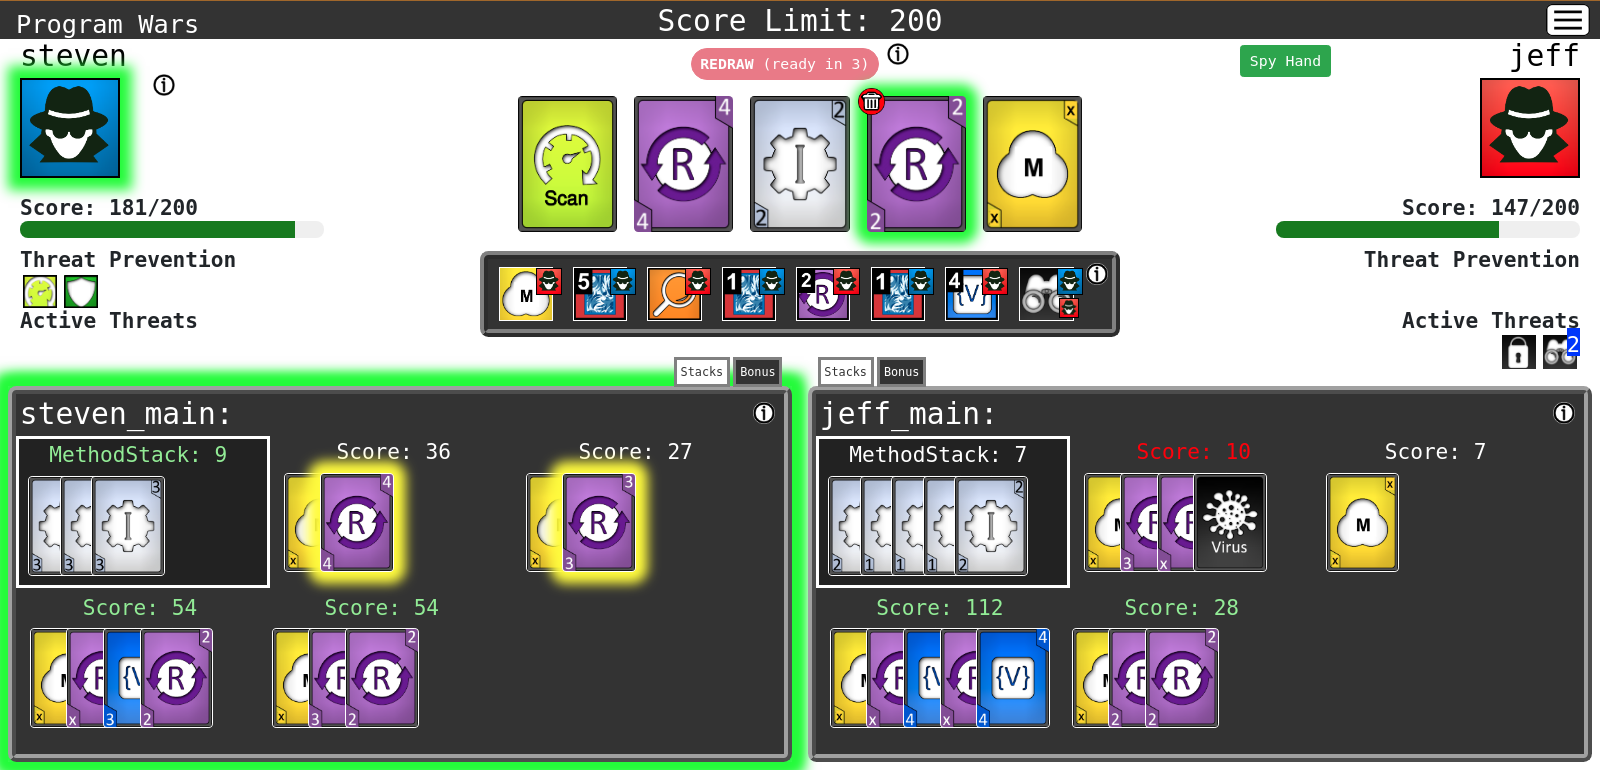
\includegraphics[width=\textwidth]{images/game.PNG}
	\caption{Partway through a game.}
	\label{fig:game}
\end{figure*}

This section presents a high-level view of the gameplay and a detailed description of the cards that teach programming fundamentals and cybersecurity in \pwTwoNS. 

\subsection{Gameplay Overview}
At the start of the game, a player can choose to play either against another human on the same computer (i.e. hot-seat play) or against provided computer opponents. \pwTwo expands the original game with two modes of gameplay: \emph{Beginner} and \emph{Standard}. For each gameplay mode, the player can choose to play with one of four different sets of cyberattack and cyberdefense cards, adding them to the game's basic deck.\footnote{A basic \gameName deck is comprised of only \Ins, \Mns, \Rns, \Vns, \Serns, \Sort and \Scan cards.}

In \B mode, only one of the two types of cyberattack cards are added to the deck - either two malware cards or two hack cards. In \Std mode, the player can choose to play with either all of the malware cards, all of the hack cards, or two different combinations of two malware and two hack cards. Each card set includes the corresponding cybersecurity cards that block the added attacks. These card sets change the gameplay difficulty through the different combinations of cybersecurity and cyberattack cards. The game uses these cards sets to progressively introduce more complicated cards. Table \ref{table:cardSets} shows the different card sets in each gameplay mode. 

\begin{table*}
	\caption{Game modes and Card sets in \pwTwoNS.}
	\begin{tabular}{|c|c|c|c|c|c|c|c|c|c|}
		\cline{1-10}
		& & \multicolumn{4}{|c|}{Beginner} & \multicolumn{4}{|c|}{Standard} \\ 
		\cline{3-10}
		Type & Card & Malware 1 & Hack 1 & Malware 2 & Hack 2 & Malware & Hack  & Combined 1 & Combined 2 \\ \hline
		\hline
		\multirow{2}{*}{Safety} & AntiVirus 	& X & & X & & X & & X & X \\ \cline{2-10}
		& Firewall 	&  & X &  & X &  & X & X & X \\ \hline \hline
		\multirow{4}{*}{Malware} & Spyware 	& X & & & & X & & X & \\ \cline{2-10}
		& Ransomware 	& X & & & & X & &  & X \\ \cline{2-10}
		& Virus		& & & X & & X & & X &  \\ \cline{2-10}
		& Trojan 		& & & X & & X & &  & X  \\ 
		\hline
		\hline
		\multirow{4}{*}{Hack} & Buffer Overflow 	& & X & & & & X & X & X \\ \cline{2-10}
		& Cross-site Scripting 	& & & & X & & X & & \\ \cline{2-10}
		& DoS Attack		& & X & & & & X & & X \\ \cline{2-10}
		& SQL Injection	& & & & X & & X & X &  \\ 
		\hline 
	\end{tabular}
	\label{table:cardSets}
\end{table*}

At the start of a game, each player is dealt five cards and the player receives another card from the deck at the end of each turn. \gameName is played in a series of rounds in which each player takes a turn to either play or discard a card from their hand, or discard and draw a new hand. A player needs to create a program that reaches the goal number of points to win the game. The points represent the total number of instructions that would be executed by the computer-based on the cards in play. Players use a variety of cards to build their program, while also fending off attacks from their opponents.

If either player has reached or exceeded the goal number of points, the game will finish at the end of the current round. This makes it possible for both players to reach the goal number of points in a game. In \B mode, the player's instruction score is all that is used to determine the winner, and players can tie. In \Std mode, bonus points are awarded for reaching specific objectives, such as the use of \R and \V cards, or ending the game without being under the influence of cyberattacks. If both players have the same total score, these bonus points are used to break ties (i.e. the player who used the most \V cards wins). If this method cannot determine a winner, the players tie.

\subsection{Gameplay Areas}

Figure \ref{fig:game} shows part of the way through a two-player game. The top right and top left corners of the screen show the status of each player. The player's name is shown along with a unique image that is highlighted with green on their turn. In Figure \ref{fig:game} it is currently Steven's turn. Under each player's image are their score and a progress bar showing their progress towards the goal number of points.\footnote{The bar is red if the player is below 50\% of the goal number of points, yellow if below 75\%, and green above 75\%.} Below the player's score is an area to show their current status effects. Status effects are represented by small icons, usually a smaller version of the image from the card that caused the effect. The \emph{Threat Prevention} section shows the current cybersecurity effects active for the player. In Figure \ref{fig:game}, Steven has a \Scan and \Anti effect active. The \emph{Active Threats} section shows any cyberattacks affecting the player. Figure \ref{fig:game} shows that Jeff has been attacked by \Ran and \Spyns. Effects that last for a specific number of turns are shown with the number of turns remaining over the top right corner. In the example game, the \Spyns 's effect on Jeff has only two turns until it expires. The status effects are added and removed as cyberattack and cybersecurity cards are played. Further details about cybersecurity and cyberattack cards and their effects are provided in Sections \ref{section:malware} and \ref{section:hacking}.

Each of the gameplay play areas contains an \emph{Information} icon (an $i$ within a circle) that when clicked on provides a short description of that play area.

\subsubsection{\Hand:}
The top of the centre area of Figure \ref{fig:game} shows the current player's hand with the player's currently selected card highlighted with green. When a card is selected, a small trash can icon appears in the upper lefthand corner of the card to allow the player to discard it. Above the cards is a button to allow the player to redraw their hand. If a player redraws their hand, they must wait for three (3) turns to do so again. In Figure \ref{fig:game}, the \emph{Redraw} button is inactive and shows that there are three turns until Steven (the current player) can use it again. 

Most cards are played by dragging the card from the hand and dropping the card where it is to be added - either the \Play or \MS areas of the \Prg. Algorithm, cybersecurity, and cyberattack cards (excluding \Vins) are played by clicking on them. When these cards are selected, a small overlay appears over the card allowing the player to make a choice. For algorithm cards, the overlay has a single button to activate the card. Safety cards have the same \texttt{Activate} button when the card can be activated. However, if the same effect is already applied to the player, then the overlay will indicate that the effect is already active, and the card will not be playable. For cyberattack cards, the overlay will give a set of buttons for valid targets of the attack. The overlay will display ``No Targets" if there are no valid targets for the attack. Some cyberattack effects will not allow certain cards to be played. Cards that cannot be played will be highlighted red while in the player's hand and will not be draggable or show an overlay when selected.

\subsubsection{\Hist:}
Below the player's hand is a visual representation of the last eight turns played. Each icon represents a card that was played. In the top right corner of each of these icons is the image of the player that played that particular card. In Figure \ref{fig:game}, the leftmost icon shows that Jeff played a \M card last turn. If a card had a target player, the target's image is placed on the bottom right corner of the card icon. This can be seen on the rightmost icon in the turn history in Figure \ref{fig:game} where it shows that Steven played a \Spy card on Jeff. Some cards may include another card or effect, such as \Scan when it removes an effect. In this case, a small icon for the card or effect included will be placed on the bottom left corner of the card image (not shown). As the game progresses, the leftmost icon is replaced by the latest card played and all icons are shifted one position to the right.

\subsubsection{\Prg:}
The bottom half of the screen represents an editor where the player builds their program. Programs are built by creating stacks of \Ins, \Mns, \R and \V cards. Each stack of cards represents a portion of the player's program. An \I or \M card can be dragged and dropped onto the \Prg~ to start a new stack. \R \\
and \V cards are played by dropping them onto an existing stack. A stack with a highlight around the top card indicates that the currently selected card can be played on that stack. If the valid stack is in the current player's \Prg, the highlight will be yellow. For cyberattack cards, such as \Vins, the valid stack will be in an opponent's \Prg and the highlight will be red. In Figure \ref{fig:game}, the currently selected \R card from Steven's hand can be played on one of the two highlighted stacks.

Each stack shows its score above it telling the player how many points that stack is contributing to the player's score. The \MS area, which is surrounded by a white border, is a special stack that only accepts instruction cards. The \MS score is the score used for the \M card, is capped at nine (9) points and the stack can hold a maximum of six (6) \I cards. Placing too many low value \I cards in a \MS can leave a player unable to reach the stack's maximum score.

The total score for a player is the sum of all of their stack scores, excluding the \MSns. Stacks with green scores indicate that the stack is complete\footnote{A stack is considered complete when it has two (2) \R cards played on it. \Rx cards only count towards completing a stack if they are paired with a \V card.} and no more cards can be added to it. A stack with a red score indicates that the stack is not contributing its full value to the total score. For example, the stack in Jeff's play area with the \Vi card on top should contribute 21 points (7 for the \M card times 3 for the \Rns-3). However, the \Vi card reduces the stack's value by half to 10 (see Section \ref{section:malware} for details). 

\subsubsection{\Goals:}
In \Std mode, a player can achieve bonus points by reaching certain goals during a game. A player's current bonus points can be seen by switching their play area to the \Bns tab. The tabs are in the centre of the screen attached to the \Prg~ of each player. This tab is not shown for a computer opponent to prevent human players from seeing a computer opponent's bonus progress. The \Bns area, shown in Figure \ref{fig:bonus}, has a set of conditional statements written in a C-like pseudocode and replaces the \texttt{True} and \texttt{False} playfields in \pwOne.

The conditional portion of the statement identifies for what the bonus is awarded. Some bonuses are for playing cards (i.e. \texttt{True} when playing a \R card), and others are for maintaining a certain status (i.e. not being affected by cyberattacks). The body of the condition shows the number of points a player will receive for satisfying the condition. If the text is red, it means the condition is not met, and the text will turn green when the player satisfies the condition. Some conditions, such as the \texttt{(no\_malware \&\& no\_hacks)} condition, may be gained or lost during the game.

At the end of each turn, the player's bonuses are re-calculated and the total bonus score is updated and shown at the top of the \Bns tab. Bonus scores are only added to the player's instruction score once the game has finished and do not apply towards reaching the goal score during the game. These bonuses are intended to help reinforce certain concepts and motivate the player towards what can be considered as good programming practices.

\begin{figure}[ht]
	\centering
	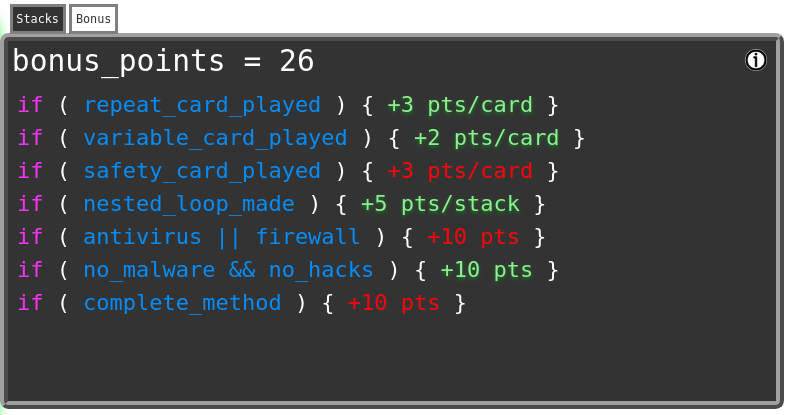
\includegraphics[width=\columnwidth]{images/objectives.PNG}
	\caption{The \Bns tab for a player.}
	\label{fig:bonus}
\end{figure}

\section{Game Cards}
The player builds their program using the basic building blocks of instructions, methods and repetition. Also, on their turn, a player can launch a cyberattack at an opponent or prepare their defence. This section describes each of the computer programming, cyberattack and cybersecurity cards in the game.

\subsection{Computer Programming}
In \pwOne the majority of cards focused on computer programming concepts, and most of these cards carry over into \pwTwoNS. 

\paragraph{\Ins, \R and \Vns:}As in actual computer programs, instructions form the backbone of the program. The \I card represents a fixed number of instructions (1, 2, or 3) and the player uses this type of card as the basis for gaining points in the game. Players can then use the \R card, which represents the concept of a loop, to further increase the overall number of instructions in their program. There are three sizes of \R cards: 2, 3, and 4. By placing a \R card on another \R card, the player can form a nested loop.\footnote{\gameName only allows nesting up to two levels to reduce the gameplay complexity and to keep scores from growing too quickly.} In addition to the fixed-size \R cards, there is also a variable \R card (called \Rxns). By itself, this card acts as a \Rns-1 card. However, the player can place a \V card on a \Rx to increases its multiplicative power. \V cards have values of 3, 4, 5 and 6. Figure \ref{fig:game} shows the example where a \M card, \R card and \V card are used.

\paragraph{\Mns:}
In \pwOneNS, the \Gr card represented the concept of a procedure, function or method in a programming language. However, the user study of \pwOne showed this card to be ineffective in conveying this concept. \pwTwo\\ replaces the \Gr card with the \M card to address this problem.

The \M card acts as a proxy for the contents of the \MS area, with the player's total score being adjusted accordingly. If a new card is added to the \MS area, the player's score will be adjusted according to the number of \M cards in the \Play area.
As with \I cards, the player can use \R and \V cards to increase the effect of a \M card. 

\subsection{Malware}
\label{section:malware}

\pwOne represented the malware cyberthreat with a single \Mal card. In \pwTwoNS, the \Mal card is replaced with cards that more directly represent four of the most common types of malware: \Spyns, \Ranns, \Vi and \Trjns. 

\paragraph{\Spyns:}
Spyware is used to gather and send information to another party without the target’s consent. The \Spy card represents this same situation in the context of the game. When a player plays a \Spy card against their opponent, a button labelled ``Spy Hand'' appears beside the opponent's name in the top portion of the screen. Clicking this button allows the attacker to be able to see the affected player's hand. The effect lasts for five turns.

\paragraph{\Ranns:}
This card's effect reflects the real-world concept of ransomware where an attacker blocks access to a target's files, such as encrypting them, and threatens to publish or delete them unless a ransom is paid. When a player plays a \Ran card on an opponent, the targeted player loses 10 points from their total score and these points are added to the attacker's score. This can result in an opponent's score becoming negative. Unlike real-world ransomware, recovering from this attack is simple, as an affected player can recover their points by either using a \Scan or \Anti card. 

\paragraph{\Vins:}
A computer virus is a computer program that replicates itself by modifying other programs. The \Vi card is used to reduce the effect of a stack of cards in the \Play area by reducing the points of a card stack. If the stack is built on an \I card, the stack's score becomes 0. If the stack is built on a \M card, the stack's score is reduced by 50\%. This adds additional motivation for the player to use the \M card. This card is the most similar to the \Mal card from \pwOneNS, where the \Mal card reduced a player's total score by 25\%.   

\paragraph{\Trjns:}
In the real world, a \Trj is a computer program that misleads users as to its real intent. When a \Trj card is played against an opponent, a random card in the opponent's hand is replaced with one that mimics it. While players can see when a \Trj is played on them they cannot tell which card has been mimicked. The actual effect of the mimic card depends on what card is replaced. \I and \M cards add the \Buf effect to the player instead of creating a new stack in the \Play area. \R and \V cards add a \Vi card to the stack where they were added. Cyberattack cards, such as \DoS or \Vins, add a \CSS to the player instead of adding a cyberattack effect to the target opponent. All cybersecurity and algorithm cards add a \Ran to the player instead of activating the expected card.

\subsection{Hacking}
\label{section:hacking}
\pwOne contained a single card, \Hackns, that represented an intrusion into a computer system. The effect of the \Hack card was to remove one of the stacks of cards on an opponent's playfield. \pwTwo refines this idea by adding specific cards to represent common ways whereby computer systems are intruded or affected by an intrusion. These four cards provide representations of the effects of four types of system attacks: causing a buffer overflow, cross-site scripting, a denial of service attack (DoS), and injection of malicious SQL code.

\paragraph{\Bufns:}
A common system attack is to send data to a program such that a memory buffer overflows and cause program instructions to be overwritten by malicious code, which is then run. In \pwTwoNS, the \Buf card prevents an opponent from playing any \Ins, \Rns, \V or \M cards for two turns. During this effect a \emph{Pass} button is added next to the \emph{Redraw} button. This allows a player to skip their turn if they cannot play any cards and do not want to discard one. The concept behind this card's effect is similar to real-world buffer overflow solutions \cite{libsafe, StackGuard}.

\paragraph{\CSSns:}
Cross-site scripting is a code injection attack. The attack happens when the victim visits a web page or web application that administers the harmful code \cite{Crosssite}. The visited web page or service acts as a carrier to deliver the malicious code to the affected browser. In \pwTwoNS, the \CSS card stops a player from playing any algorithm or cyberattack cards for two turns. This effect also adds a \emph{Pass} button above the \Hand. The concept behind this card is to make a player familiar with this type of attack by preventing the advantages given by algorithm and cyberattack cards.

\paragraph{\DoSns:}
A Denial of Service (DoS) attack occurs when a computer system connected to a network is intentionally flooded with requests so that the system can no longer handle legitimate requests. In \pwTwoNS, the \DoS card prevents a player from redrawing new cards at the end of their turn. The effect also adds a \emph{Pass} button above the \Hand~ and disables the \emph{Redraw} button. The effect lasts for three turns resulting in the player having fewer cards in their hand to choose from until the effect ends.

\paragraph{\SQLns:}
In an SQL injection attack, malicious SQL code is entered into a data field such that the code is run on a backend database. The result of such an attack is to obtain information that was not intended to be disclosed or delete and/or corrupt the data in the database. In \pwTwoNS, the \SQL card can be used to slow down the progress of an opponent by reducing the total of the \MS area by two points. The effect lasts until removed by a \Fire or \Scan card. The concept behind this card is that of infiltration of a program's method by malicious code. 

\subsection{Cyberdefense:}
\pwOne provided three cards for cyberdefense. Two of the cards were \emph{permanent} cards, meaning that they remained on a player's playfield when played, and were referred to as \emph{Safeties}. The first of these cards was the \Anti card which prevented the \Mal card from being played on a player. The second of these cards was the \Fire card which protected against the \Hack card. The third card was the \Over card, which combated the \Mal card by increasing the player's total score by 25\%. However, it was observed that the \Over effect didn't match well with real-world cybersecurity concepts and was removed in \pwTwoNS.  

\pwTwo continues the use of the two safety cards, \Anti and \Firens, and adds a new one-time-use cyberdefense card called \Scanns. 

\paragraph{\Scanns:}
The \Scan card represents the action of a user explicitly scanning all of their files to find any infected items using an antivirus tool. If the player is under the influence of either a malware or a hack card, then the \Scan card allows the players to choose a single effect to remove. If the player is not under the influence of a cyberattack card, the effect is saved until the player is attacked, at which time the cyberattack is neutralized and the \Scan effect is removed.

\paragraph{\Antins:}
An antivirus program is a program or set of programs designed to prevent, search for, detect, and remove malware from a computer system. The \Anti card reflects this real-world tool by protecting a player from the effect of any of the malware attack cards. If the player is already under the effect of one or more malware cards, all of the effects are removed when this card is played. Unlike the \Scan card, the effect of this card is permanent once it is played, thereby protecting the player from any future malware card attacks. 

\paragraph{\Firens:}
A firewall is a network security device that controls incoming and outgoing network traffic and grants or prevents data packets based on a set of security rules, thereby protecting a computer system from various intrusion attacks. Like the \Anti card, the \Fire card reflects this real-world tool by preventing hack cards from being played on the player. Similar to the \Anti card, if the player is affected by any hack cards, these effects are removed. The effect of this card is also permanent once played.

\subsection{Algorithms/Library Functions:}
The use of algorithms, often from libraries, is an essential part of computer programming. Two key categories of algorithms are searching and sorting, and both of these are introduced in \pwTwoNS.

\paragraph{\Sortns:}
Sorting is the arrangement of items into an ordered sequence. In \pwTwoNS, the \Sort card allows a player to rearrange the top five (5) cards of the deck into whatever order they choose. This allows a player to control what cards players will draw for the next five turns, three cards for the player, and two for their opponent. When the card is played, an overlay is opened showing the top five cards and the player can drag and drop cards to reorder them.

\paragraph{\Serns:}
Searching is the process of locating a particular element in a given set of elements. In \pwTwoNS, the \Ser card allows a player to search for a specific card within the top ten (10) cards of the deck. Playing the card results in an overlay being opened that shows these cards and the player selects one to immediately put into their hand for their next turn.


\section{Conclusion}
This paper presented an evolution of the game elements and concepts introduced by \pwOne \cite{anvikPW}. Regarding programming concepts, the \Gr card was changed to the \M card to better represent procedures, functions and methods in programs. Also, the the conditional statement concept was made more explicit with the use of gameplay goals. Similarly, the general cybersecurity concepts in \pwOne were specialized in \pwTwoNS. Finally, \pwTwo introduced the concepts of algorithms through the addition of the \Ser and \Sort cards. Regarding gameplay, two modes of play (\B and \StdNS) were introduced to provide a learning path for players, and the user interface was revised to provide more player and game information.  

In the near future, we will be conducting a user study to investigate the effects of \pwTwo on learning fundamental concepts of computer programming and cybersecurity. Also, the next version of \gameName will introduce a gameplay mode focused on teaching the Software Development Lifecycle (SDLC) and the Agile software development methodology. 
%\section{Acknowledgements}
We acknowledge the efforts of Shaun Cullen, Lance Chisholm, Dustin Fowler, Joshua Vandenhoek, and Jonathan Vos for the initial implementation of \pwOne as a course project, and the efforts of Austin Ball, Vincent Cote and Jace Riehl towards improving \pwOne as undergraduate summer students. This work was partially funded by NSERC.


\bibliographystyle{ACM-Reference-Format}
\balance
\bibliography{paper_JSEET_2021}

\end{document}
